% !TeX root = RJwrapper.tex
\title{\pkg{fcaR}, Formal Concept Analysis with R}
\author{by Pablo Cordero, Manuel Enciso, Domingo López-Rodríguez, and Ángel
Mora}

\maketitle

\abstract{%
Formal concept analysis (FCA) is a solid mathematical framework to
manage information based on logic and lattice theory. It defines two
explicit representations of the knowledge present in a dataset as
concepts and implications. This paper describes an R package called \CRANpkg{fcaR}
that implements FCA's core notions and techniques. Additionally, it
implements the extension of FCA to fuzzy datasets and a simplification
logic to develop automated reasoning tools. This package is the first to
implement FCA techniques in R. Therefore, emphasis has been put on
defining classes and methods that could be reusable and extensible by
the community. Furthermore, the package incorporates an interface with
the \CRANpkg{arules} package, probably the most used package regarding association
rules, closely related to FCA. Finally, we show an application of
the use of the package to design a recommender system based on logic for
diagnosis in neurological pathologies.
}

\hypertarget{introduction}{%
\section{Introduction}\label{introduction}}

The main goal of knowledge retrieval and knowledge discovery systems is
to extract hidden patterns, trends, behaviours, or rules to solve
large-impact real-world problems. Usually, these problems present
heterogeneous data sources and are at the core of more general decision
processes.

A fundamental principle is that the extracted knowledge should provide
some understanding of the analyzed data. As computational systems get in
critical and sensitive areas such as medicine, the justice system or
financial markets, the knowledge becomes much more relevant to make
predictions or recommendations or to detect common interest groups or
leaders. However, in many cases, the inability of humans to understand
the extracted patterns seems problematic.

To represent and retrieve knowledge from datasets, it has become more
important to use formal methods based on logic tools. The formal
representation of knowledge and the use of logic tools are more suitable
for providing understandable answers. Therefore, it can help avoid the
lack of interpretability and explainability of the results.

In particular, formal concept analysis (FCA)
\citep{wille1982restructuring, Ganter1999} is a well-founded
mathematical tool, based on lattice theory and logic, which can retrieve
and store the knowledge in the form of concepts (analogous to closed
itemsets in transactional databases) and implications (association rules
with confidence 1). From this perspective, FCA constitutes a framework
that complements and extends the study of exact and approximate
association rules.

The origins of FCA were devoted to the study of binary datasets (formal
contexts) where variables are called attributes. A relevant extension of
FCA uses fuzzy sets~\citep{BeVyAddgI, BeVyAddgII} to model
real-world problems since datasets may contain imprecise, graded or
vague information that is not adequately represented as binary values.
The fuzzy extension can also model problems with numerical and
categorical attributes since these can be scaled to a truth value
describing the degree of fulfilment of the attribute.

Some authors have considered the use of FCA in machine learning.
\citet{Kuznetsov04} relates FCA to some mathematical models of machine
learning. \citet{Ignatov2015} summarizes the main topics in machine
learning and data mining where FCA has been applied: frequent itemset
mining and association rules to make classification and clustering. A
closer approach appears in \citet{Trabelsi17}, where a method for
supervised classification based on FCA is used. The authors extract
rules based on concepts generated previously from data. These rules are
used to compute the closure of a set of attributes to obtain a
classification rule.

From a dataset, FCA can establish maximal clusters, named concepts,
between objects and attributes. Each cluster consists of objects having
common properties (attributes), which are only fulfilled for these
objects. The hierarchy between the concepts and relationships between
the attributes (rules or implications) are computed with the same
computational cost in FCA.

Among all the techniques used in other areas to extract knowledge, we
emphasize using rules for its theoretical and practical interest. The
notion of if-then rules, with different names, appears in several areas
(databases, machine learning, data mining, formal concept analysis) as a
relationship between attributes, called items, properties or atomic
symbols regarding the domain. Nowadays, the number of rules extracted
even from medium-sized datasets is enormous in all these areas.
Therefore, the intelligent manipulation of these rules to reason with
them is a hot topic to be explored.

In this direction, \citet{Cordero2002} introduced a logic, named
simplification logic for functional dependencies (\(SL_{FD}\)), firmly
based on a simplification rule, which allows us to narrow the functional
dependency set by removing redundant attributes. Although the semantic
of implications or if-then rules in other areas are different, the logic
can be used too.

Using directly \(SL_{FD}\), some automated deduction methods directly
based on this inference system have been developed for classical systems
and fuzzy systems
\citep{mora_efficient_2004, Cordero2012, Mora2012, cla2014, Lorenzo2015}.

In the fuzzy framework, several approaches to the definition of fuzzy
implications (functional dependencies, rules) are proposed in the
literature, see \citet{JEZKOVA2017} for a survey. Our work considers
that the definition of graded implication proposed by
\citet{BeVyAddgI, BeVyAddgII} generalizes all the previous definitions.
Furthermore, for this general definition of graded implications, an
axiomatic system named FASL (fuzzy attribute simplification logic) was developed by \citet{belohlavek2016automated}, becoming a helpful
reasoning tool. Note that FASL is a generalization of \(SL_{FD}\) to the
fuzzy framework.

The core of our proposal is to provide a user-friendly computational
interface to the principal operators and methods of fuzzy FCA, including
the mentioned logic tools. This interface is easy to extend to new
functionalities and incorporate new methods, such as minimal generators
or the computation of different implication bases quickly. The operators
and methods implemented are designed to work in the general fuzzy
setting, but they are also applicable in the classical binary case.

Thus, the focus of our proposal, the \pkg{fcaR} package, is to
provide easy access to formal methods to extract all the implicit
knowledge in a dataset in the form of concepts and implications, working
natively with fuzzy sets and fuzzy implications. Our goal is to provide
a unified computational framework for the theoretically-oriented FCA
users to develop, test, and compare new methods and knowledge extraction
strategies.

Other objectives of this work include presenting an FCA-based tool for
knowledge discovery accessible to other scientific communities, allowing
for the development of new packages in other fields using FCA
techniques, especially in the construction of recommendation systems.

The work is organized as follows: Section~\nameref{definitions} begins
with a brief look of FCA and Simplification Logic.
Section~\nameref{related} presents other software libraries that
implement FCA or related paradigms' core notions. In
Section~\nameref{design}, an explanation of the data structures, classes
and constructor methods is covered. Section~\nameref{fcaR} shows how to
use the package, describing the implemented FCA methods and the use of
the simplification logic. In Section~\nameref{examples}, a real
application of the package in developing a recommender system is
illustrated. Finally, some conclusions and future works are presented in
Section~\nameref{conclusions}.

\hypertarget{definitions}{%
\section{Background on FCA}\label{definitions}}

In this section, we present the basic notions in the FCA framework using
a running example (see Table~\ref{tab:fc}). Note that the package
incorporates the main methods in FCA that appear in this summary. Since
the formal study of FCA is not the main scope of this work, we recommend
the reference \citep{ganter2016conceptual} for further details of this
framework.

\begin{table} \centering \begin{tabular}{lcccc}
\toprule
 & P1 & P2 & P3 & P4\\
\midrule
O1 & 0 & \sfrac{1}{2} & \sfrac{1}{2} & \sfrac{1}{2}\\
O2 & \sfrac{1}{2} & 1 & 0 & 1\\
O3 & \sfrac{1}{2} & 1 & 0 & 1\\
O4 & 0 & \sfrac{1}{2} & 1 & \sfrac{1}{2}\\
\bottomrule
\end{tabular} \caption{\label{tab:fc}A sample formal context. The attributes are P1 to P4 and the objects are named O1 to O4.} \end{table}

A \dfn{formal context} is a triple \((G, M, I)\), where \(G\) is a set
of objects, \(M\) is a set of attributes and \(I\) is a fuzzy relation
between objects and attributes, where \(I(x, y) \in [0, 1]\) means the
truth value to which object \(x\) possesses attribute \(y\), indicating
\(I(x,y) = 0\) the absence of attribute or property \(y\) in object
\(x\).

The meaning of each entry in the table is the extent to which an object
possesses the attribute in the corresponding column. In the example
shown in Table~\ref{tab:fc}, the object named O4 fully possesses
attribute P3 and possesses P2 and P4 only to degree 50\%.

In the remaining of this paper, we will use the notation \(^{d\!}/a\) to
indicate the presence of attribute \(a\) with degree \(d\).

\hypertarget{derivation-operators}{%
\subsection{Derivation operators}\label{derivation-operators}}

Given a fuzzy set of objects \(\mathcal{S}\), we can compute its
\dfn{intent} as the set of attributes that are shared by all objects in
\(\mathcal{S}\). Analogously, we define the \dfn{extent} of a set
\(\mathcal{T}\) of attributes as the set of objects which have
\emph{all} the attributes in \(\mathcal{T}\).

In the above example, for
\(S=\)\ensuremath{\left\{\mathrm{O1},\, \mathrm{O2}\right\}}, we have
\(\text{intent}(S)=\)\ensuremath{\left\{{^{0.5}}\!/\mathrm{P2},\, {^{0.5}}\!/\mathrm{P4}\right\}}
because \(I(\mathrm{O1}, \mathrm{P2}) = 0.5\),
\(I(\mathrm{O1}, \mathrm{P4}) = 0.5\),
\(I(\mathrm{O2}, \mathrm{P2}) = 1\) and
\(I(\mathrm{O2}, \mathrm{P4}) = 1\).

The operator \(\phi\) defined by
\(\phi(T) = \text{intent}(\text{extent}(T))\) is a closure operator and
a set of attributes \(\mathcal{T}\) is called \dfn{closed} if
\(\mathcal{T} = \phi(\mathcal{T})\). In our example,
\(\phi(\ensuremath{\left\{{^{0.5}}\!/\mathrm{P1}\right\}}) = \ensuremath{\left\{{^{0.5}}\!/\mathrm{P1},\, \mathrm{P2},\, \mathrm{P4}\right\}}\),
meaning that \emph{every object} that has P1 with degree at least 0.5,
also has all the attributes
\ensuremath{\left\{\mathrm{P2},\, \mathrm{P4}\right\}}. When
\(\mathcal{T}\) is closed, the pair
\((\text{extent}(\mathcal{T}), \mathcal{T})\) is called a \dfn{concept}.

In general, a concept \((A, B)\), where \(A\) is a set of objects, and
\(B\) is a set of attributes, means that the only attributes shared by
all objects in \(A\) are those in \(B\), and the only objects having all
attributes in \(B\) are those in \(A\). This property makes \((A, B)\) a
\emph{maximal rectangular cluster} in the dataset, with a strong
dependence between the objects in \(A\) and the attributes in \(B\). In
the formal context represented in Table~\ref{tab:fc}, the pair
\ensuremath{\left(\ensuremath{\left\{\mathrm{O2},\, \mathrm{O3}\right\}}, \ensuremath{\left\{{^{0.5}}\!/\mathrm{P1},\, \mathrm{P2},\, \mathrm{P4}\right\}}\right)}
is a concept, because
\(\text{extent}(\ensuremath{\left\{{^{0.5}}\!/\mathrm{P1},\, \mathrm{P2},\, \mathrm{P4}\right\}})=\ensuremath{\left\{\mathrm{O2},\, \mathrm{O3}\right\}}\)
and
\(\text{intent}(\ensuremath{\left\{\mathrm{O2},\, \mathrm{O3}\right\}})=\ensuremath{\left\{{^{0.5}}\!/\mathrm{P1},\, \mathrm{P2},\, \mathrm{P4}\right\}}\),
i.e.~a fixpoint is achieved.

In FCA, using these derivation operators, two operations can be used to
reduce a formal context:

\begin{itemize}
\tightlist
\item
  \dfn{Clarification}, which is the removal of duplicated rows (objects)
  and columns (attributes) of the formal context since duplicates do not
  contribute knowledge to the context.
\item
  \dfn{Reduction}, which removes attributes that can be expressed as the
  closure of other attributes.
\end{itemize}

These two operations remove redundancies in the formal context without
affecting the knowledge contained in it. Many of the subsequent
operations in FCA have high computational complexity, and clarifying and
reducing a formal context may reduce the computational time of posterior
operations.

\hypertarget{the-concept-lattice}{%
\subsection{The concept lattice}\label{the-concept-lattice}}

The \dfn{concept lattice} of a formal context is the set of all
concepts, with the partial order \(\le\) defined as follows: for two
concepts \((A_1, B_1)\) and \((A_2, B_2)\), we say that
\((A_1, B_1) \le (A_2, B_2)\) if and only if
\(A_1 \subseteq A_2 \iff B_2 \subseteq B_1\). For instance,
\(\ensuremath{\left(\ensuremath{\left\{{^{0.5}}\!/\mathrm{O2},\, {^{0.5}}\!/\mathrm{O3}\right\}}, \ensuremath{\left\{\mathrm{P1},\, \mathrm{P2},\, \mathrm{P4}\right\}}\right)}  \le \ensuremath{\left(\ensuremath{\left\{\mathrm{O2},\, \mathrm{O3}\right\}}, \ensuremath{\left\{{^{0.5}}\!/\mathrm{P1},\, \mathrm{P2},\, \mathrm{P4}\right\}}\right)}\),
since their intents verify
\(\ensuremath{\left\{{^{0.5}}\!/\mathrm{P1},\, \mathrm{P2},\, \mathrm{P4}\right\}} \subseteq \ensuremath{\left\{\mathrm{P1},\, \mathrm{P2},\, \mathrm{P4}\right\}}\).

This order (or precedence) relationship induces a hierarchy of concepts,
which can be graphically represented in the Hasse diagram
\citep{birkhoff1940lattice} of the partially ordered set of concepts. In
Figure~\ref{fig:lattice}, we find the Hasse diagram corresponding to our
running example.

\begin{figure}

\centering 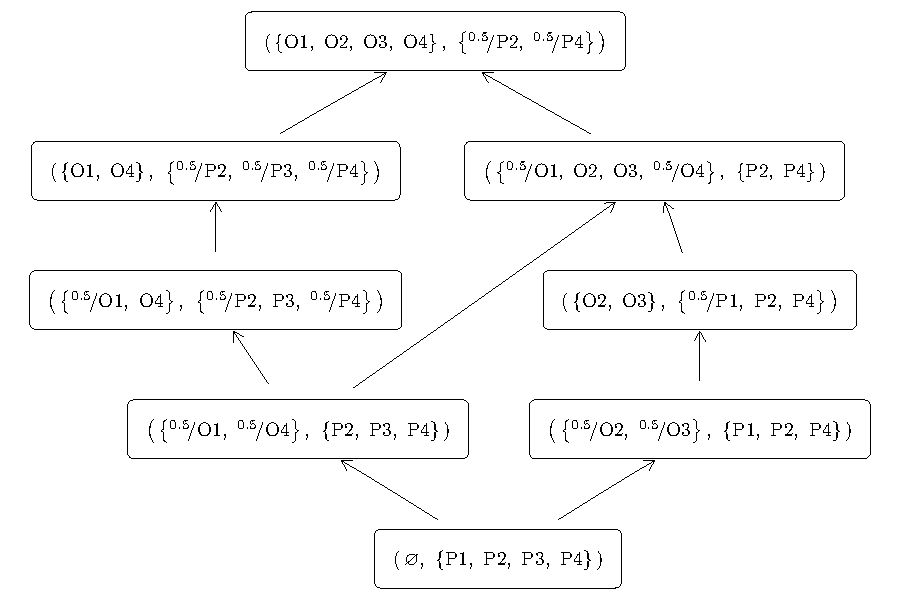
\includegraphics[width=0.5\textwidth]{fig-lattice.pdf}

\caption{\label{fig:lattice}Concept lattice for the context in Table \ref{tab:fc}. Arrows indicate the direction of the order relationship between concepts.}
\end{figure}

From the concept lattice and the order relationship, we can define
notions as \dfn{subconcept}, \dfn{superconcept}, \dfn{infimum} and
\dfn{supremum} of a set of concepts.

Notably, there are the \dfn{irreducible elements}, for the infimum
(meet) or the supremum (join) operators, which, in the lattice, are
shown as those elements with only one arrow departing or arriving at
them, respectively. These elements are essential since one can
reconstruct the whole lattice by operating with these elements.

The \dfn{standard context} for a given formal context \(\mathbb{K}\) is
another formal context \((\mathcal{J}, \mathcal{M}, \le)\), where
\(\mathcal{J}\) and \(\mathcal{M}\) are the sets of join- and
meet-irreducible elements of \(\mathbb{K}\) and \(\le\) is the partial
order defined in the concept lattice. This standard context has a
concept lattice isomorphic to that of \(\mathbb{K}\).

\hypertarget{implications-and-logic}{%
\subsection{Implications and logic}\label{implications-and-logic}}

The knowledge stored in a formal context can also be represented as a
set of implications, which are expressions of the form
\(A\Rightarrow B\) where \(A\) and \(B\) are sets of attributes or
items, indicating that, for every object in which the set of attributes
\(A\) is present, also \(B\) is present. This interpretation is similar
to the one defined in data mining/machine learning over the so-named
association rules. The confidence (a well-known estimator of the rules'
quality) has value 1 in all the implications.

For instance
\(\left\{{^{0.5}}\!/\mathrm{P1}\right\}\Rightarrow\left\{\mathrm{P4}\right\}\)
is a valid implication in the previous example, having the following
interpretation: when the attribute \(\mathrm{P1}\) has degree at least
\(0.5\) then we have \(\mathrm{P4}\) with degree \(1\).

The \dfn{Duquenne-Guigues basis} of implications
\citep{guigues1986familles} is a set of valid implications from which
all other valid implications can be deduced. The Duquenne-Guigues basis
in our example is given by:

\begingroup\footnotesize

\begin{longtable*}{rrcl}
1: &\ensuremath{\varnothing}&\ensuremath{\Rightarrow}&\ensuremath{\left\{{^{0.5}}\!/\mathrm{P2},\, {^{0.5}}\!/\mathrm{P4}\right\}}\\
2: &\ensuremath{\left\{{^{0.5}}\!/\mathrm{P2},\, \mathrm{P4}\right\}}&\ensuremath{\Rightarrow}&\ensuremath{\left\{\mathrm{P2}\right\}}\\
3: &\ensuremath{\left\{\mathrm{P2},\, {^{0.5}}\!/\mathrm{P4}\right\}}&\ensuremath{\Rightarrow}&\ensuremath{\left\{\mathrm{P4}\right\}}\\
4: &\ensuremath{\left\{\mathrm{P2},\, {^{0.5}}\!/\mathrm{P3},\, \mathrm{P4}\right\}}&\ensuremath{\Rightarrow}&\ensuremath{\left\{\mathrm{P3}\right\}}\\
5: &\ensuremath{\left\{{^{0.5}}\!/\mathrm{P1},\, {^{0.5}}\!/\mathrm{P2},\, {^{0.5}}\!/\mathrm{P4}\right\}}&\ensuremath{\Rightarrow}&\ensuremath{\left\{\mathrm{P2},\, \mathrm{P4}\right\}}\\
6: &\ensuremath{\left\{{^{0.5}}\!/\mathrm{P1},\, \mathrm{P2},\, \mathrm{P3},\, \mathrm{P4}\right\}}&\ensuremath{\Rightarrow}&\ensuremath{\left\{\mathrm{P1}\right\}}\\
\end{longtable*}\endgroup

In \citet{Cordero2002}, the simplification logic, denoted as
\(SL_{FD}\), was introduced as a method to manipulate implications
(functional dependencies or if-then rules), removing redundancies or
computing closures of attributes. This logic is equivalent to
Armstrong's Axioms \citep{Armstrong1974}, which are well known from the
80s in databases, artificial intelligence, formal concept analysis, and
others. The axiomatic system of this logic considers reflexivity as the
axiom scheme
\begin{center}
{\scriptsize \tt{[Ref]}}\quad {\footnotesize $\displaystyle\frac{A\supseteq B}{A \Rightarrow B}$ }
\end{center}
together with the following inference rules called fragmentation,
composition and simplification, respectively, which are equivalent to
the classical Armstrong's axioms of augmentation and, more importantly,
transitivity.

\begin{center}
{\scriptsize \tt{[Frag]}}\ {\footnotesize $\displaystyle\frac{A\Rightarrow B\cup C}{A\Rightarrow B}$}
 \quad
{\scriptsize \tt{[Comp]}}\  {\footnotesize $\displaystyle\frac{A\Rightarrow B,\ C \Rightarrow D}{A\cup C \Rightarrow B\cup D}$ } \quad
{\scriptsize \tt{[Simp]}}\  {\footnotesize $\displaystyle\frac{A\Rightarrow B,\ C \Rightarrow D}{A\cup(C\smallsetminus B)\Rightarrow(D\smallsetminus B)}$}
\end{center}

The main advantage of \(SL_{FD}\) with respect to Armstrong's Axioms is
that the inference rules may be considered as equivalence rules, (see the work by
\citet{Mora2012} for further details and proofs), that is, given a set
of implications \(\Sigma\), the application of the equivalences
transforms it into an equivalent set. In the package presented in this
paper, we develop the following equivalences:

\begin{enumerate}
\item  Fragmentation Equivalency {\bf [FrEq]}:
$\{A\Rightarrow B\}\equiv\{A\Rightarrow B\smallsetminus A\}$.
\item  Composition Equivalency {\bf [CoEq]}:
$\{A\Rightarrow B, A\Rightarrow C\}\equiv\{A\Rightarrow B{\cup} C\}$.
\item Simplification Equivalency {\bf [SiEq]}:
If $A\subseteq C${,} then\\[2mm]
\centerline{$
\{A\Rightarrow B, C \Rightarrow D\}\equiv  \{A\Rightarrow B, { A\cup(}C\smallsetminus B)\Rightarrow D\smallsetminus B\}$}
\item {Right-Simplification Equivalency {\bf [rSiEq]}:
If $A\subseteq D$, then\\[2mm]
\centerline{$
 \{A\Rightarrow B, C\Rightarrow B\cup D\}\equiv \{A\Rightarrow B, C \Rightarrow D\}$}}
\end{enumerate}

Usually, many areas, the implications have always atomic attributes on
the right-hand side. We emphasize that this logic can manage
\emph{aggregated} implications, i.e.~the implications' consequents do
not have to be singletons. This represents an increase of the logic
efficiency.

This logic removes attribute redundancies in some of the implications in
the Duquenne-Guigues basis presented before. Particularly, the
implications with numbers 2, 3, 4, 5 and 6 are simplified to:
\begingroup\footnotesize

\begin{longtable*}{rrcl}
2: &\ensuremath{\left\{\mathrm{P4}\right\}}&\ensuremath{\Rightarrow}&\ensuremath{\left\{\mathrm{P2}\right\}}\\
3: &\ensuremath{\left\{\mathrm{P2}\right\}}&\ensuremath{\Rightarrow}&\ensuremath{\left\{\mathrm{P4}\right\}}\\
4: &\ensuremath{\left\{{^{0.5}}\!/\mathrm{P3},\, \mathrm{P4}\right\}}&\ensuremath{\Rightarrow}&\ensuremath{\left\{\mathrm{P3}\right\}}\\
5: &\ensuremath{\left\{{^{0.5}}\!/\mathrm{P1}\right\}}&\ensuremath{\Rightarrow}&\ensuremath{\left\{\mathrm{P4}\right\}}\\
6: &\ensuremath{\left\{{^{0.5}}\!/\mathrm{P1},\, \mathrm{P3}\right\}}&\ensuremath{\Rightarrow}&\ensuremath{\left\{\mathrm{P1}\right\}}\\
\end{longtable*}\endgroup

One of the primary uses of a set of implications is computing the
closure of a set of attributes, the maximal fuzzy set that we can arrive
at from these attributes using the given implications.

The importance of computing the closure from implications is because
implications can be managed using logic tools. They formally describe
the knowledge existing in the dataset; thus, the user can forget about
the original \textit{dataset}. In this sense, it is similar to
supervised Machine Learning techniques.

The algorithm to compute the closure \citep{Mora2012} is based on the
classical \textsc{closure} algorithm
\citep{maier1983theory, ganter2016conceptual}. After each pass over the
set of implications, instead of simply removing the implications used in
the step, the simplification rule substitutes the implications by others
equivalent but simpler, with fewer attributes. In the binary case, the
reduced set of implications does not reference any attribute in the
computed closure. A detailed description of the procedure is presented
in Algorithm~\ref{algo:closure}.

\begin{algorithm}[h]
\small
\DontPrintSemicolon
\SetAlgoLined
\SetKwInOut{Input}{Input}\SetKwInOut{Output}{Output}
\Input{$X$: attribute set; $\Gamma$: set of implications}
\Output{$X^+$: the closure of $X$ with respect to $\Gamma$; $\Gamma'$: the simplified set of implications}
\BlankLine
$\Gamma' := \Gamma \cup \{\varnothing\Rightarrow X\}$\;
$X_{\mathrm{new}} := X$\;
$X_{\mathrm{old}} := X$\;
\Repeat{$X_{\mathrm{old}} = X_{\mathrm{new}}$}{
    Replace $\{\varnothing\Rightarrow X_{\mathrm{old}}\}$ with $\{\varnothing\Rightarrow X_{\mathrm{new}}\}$ in $\Gamma'$\;
    $X_{\mathrm{old}} = X_{\mathrm{new}}$\;

\For{\text{each} $A\Rightarrow B\in\Gamma'\setminus\{\varnothing\Rightarrow X_{\mathrm{new}}\}$}{

\If{$A\subseteq X_{\mathrm{new}}$}{
   Replace $\{\varnothing\Rightarrow X_{\mathrm{new}}\}$ with $\{\varnothing\Rightarrow X_{\mathrm{new}}\cup B\}$\;
   $X_{\mathrm{new}} := X_{\mathrm{new}}\cup B$\;
}
\If{$B\subseteq X_{\mathrm{new}}$}{
    Remove $A\Rightarrow B$ from $\Gamma'$\;
}
\If{$A\cap X_{\mathrm{new}}\ne\varnothing$ \text{or} $B\cap X_{\mathrm{new}}\ne\varnothing$}{
    Replace $A\Rightarrow B$ with $A\setminus X_{\mathrm{new}}\Rightarrow B\setminus X_{\mathrm{new}}$\;
}

}

}

\Return{$X^+$ and $\Gamma'$}

\caption{$SL_{FD}$ closure\label{algo:closure}}
\end{algorithm}

For instance, the closure of
\(S = \ensuremath{\left\{{^{0.5}}\!/\mathrm{P2}\right\}}\) with this
algorithm is
\(S^+ = \ensuremath{\left\{{^{0.5}}\!/\mathrm{P2},\, {^{0.5}}\!/\mathrm{P4}\right\}}\)
(this means that all objects that have all the attributes in \(S\), also
have those in \(S^+\)). The simplification logic leads us to a reduced
set of implications \(\Gamma'\): \begingroup\footnotesize

\begin{longtable*}{rrcl}
1: &\ensuremath{\left\{\mathrm{P4}\right\}}&\ensuremath{\Rightarrow}&\ensuremath{\left\{\mathrm{P2}\right\}}\\
2: &\ensuremath{\left\{\mathrm{P2}\right\}}&\ensuremath{\Rightarrow}&\ensuremath{\left\{\mathrm{P4}\right\}}\\
3: &\ensuremath{\left\{\mathrm{P2},\, {^{0.5}}\!/\mathrm{P3},\, \mathrm{P4}\right\}}&\ensuremath{\Rightarrow}&\ensuremath{\left\{\mathrm{P3}\right\}}\\
4: &\ensuremath{\left\{{^{0.5}}\!/\mathrm{P1}\right\}}&\ensuremath{\Rightarrow}&\ensuremath{\left\{\mathrm{P2},\, \mathrm{P4}\right\}}\\
5: &\ensuremath{\left\{{^{0.5}}\!/\mathrm{P1},\, \mathrm{P2},\, \mathrm{P3},\, \mathrm{P4}\right\}}&\ensuremath{\Rightarrow}&\ensuremath{\left\{\mathrm{P1}\right\}}\\
\end{longtable*}\endgroup

One can interpret these implications as the knowledge in the original
implications if the attributes in \(S\) are not considered (formally,
this is equivalent to suppose that \(\varnothing\Rightarrow S\) is
true). In the example, if, in addition to having
\ensuremath{\left\{{^{0.5}}\!/\mathrm{P2}\right\}}, we have
\(\{\mathrm{P1}\}\) with degree \(0.5\), we can infer that
\(\{\mathrm{P2}\}\) and \(\{\mathrm{P4}\}\) are fully present, by
implication number 4.

\hypertarget{related}{%
\section{Related works}\label{related}}

The package presented in this paper has been developed in the R
language. In recent years, R has lived a \emph{remarkable revolution}
caused in part by an increasing user community from many different
scientific fields. This has led to the development of reproducible
research tools, e.g., \CRANpkg{rmarkdown} \citep{rmarkdown}, and tools
to connect and interact with other programming languages, with packages
like \CRANpkg{Rcpp} \citep{rcpp} or \CRANpkg{reticulate}
\citep{reticulate}. Besides, the development of a game-changer
programming paradigm with \emph{tidy} principles  has provided a significant
impact on R's usability, see the
\CRANpkg{tidyverse} of \citet{tidyverse}.

These facts have transformed R from a purely statistical language into
one of the most popular languages in data science, machine learning,
data mining or visualization. In R, there are multiple packages to
perform data mining and machine learning tasks. However, only a few of
them are focused on formal methods that can model and extract knowledge
in the form of implications and rules on fuzzy sets and operate on them
using logic tools.

The \pkg{arules} package by \citet{Hashler} provides the
infrastructure for representing, manipulating and analyzing transaction
data and patterns (frequent itemsets and association rules) in
\emph{binary} settings. The \CRANpkg{frbs} package \citep{frbs} presents
an implementation of various learning algorithms based on fuzzy
rule-based systems (FRBSs) for dealing with classification and
regression tasks. The \CRANpkg{RKEEL} package \citep{rkeel} is an R
interface to KEEL, a popular Java software for a large number of
different knowledge data discovery tasks. It can extract association
rules from numerical datasets, but variables are discretized or
categorized first.

It must be noted that none of the previous approaches uses logic tools
to infer knowledge from the extracted rules and implications. Also, the
support for fuzzy sets is minimal, and none of them implements the core
notions of FCA.

Since the \pkg{arules} package has become a \emph{de facto} standard,
one of the critical points in our proposal's design has been to get
\pkg{fcaR} easily integrated with \pkg{arules}.

In other programming languages, several libraries are implementing FCA
methods. Some of the most used libraries are focused on computing the
concept lattice and provide a graphical interface to operate with the
formal context and the concept lattice: ToscanaJ \citep{Becker_2005} and
Galicia \citep{valtchev2003galicia}. Other tools, such as Concept
Explorer (ConExp) \citep{yevtushenko2000system}, with its new versions
ConExp NG and ConExp FX, besides their graphical capabilities, implement
the core FCA algorithms and operations: context editing, building
concept lattices, finding bases of implications and association rules,
for instance.

The two most recent and fully-featured libraries are conexp-clj
\citep{hanika2019conexp} and GALACTIC \citep{demko2020galactic},
focusing on their extensibility and addition of multiple new algorithms,
including the implementation of closure operators and methods based on
implications.

In Table~\ref{tab:comparison}, we present a comparison of the main
features present in each of these libraries.

\begin{table}
\footnotesize\center
\begin{tabular}{l|c@{\,\,}c@{\,\,}c@{\,\,}c@{\,\,}c@{\,\,}c@{\,\,}c@{\,\,}c@{\,\,}c}
 & ToscanaJ & ConExp & conexp-clj & Galicia & GALACTIC & \CRANpkg{arules} & \CRANpkg{RKEEL} & \CRANpkg{frbs} & \CRANpkg{fcaR}\\
\hline
Programming language & Java & Java & Clojure & Java & Python & R & R & R & R \\
Context operations &  & $\times$ & $\times$ & $\times$ & $\times$ & &  &  & $\times$\\
Context visualization &  & $\times$ & $\times$ & $\times$ & $\times$ &  &  &  & $\times$\\
Lattice computation &  & $\times$ & $\times$ & $\times$ & $\times$ &  &  &  & $\times$\\
Lattice operations & $\times$ & $\times$ & $\times$ & $\times$ & $\times$ &  &  &  & $\times$\\
Lattice visualization & $\times$ & $\times$ & $\times$ & $\times$ & $\times$ &  &  &  & $\times$\\
Implication basis computation &  & $\times$ & $\times$ &  & $\times$ &  &  &  & $\times$\\
Association rules computation &  & $\times$ & $\times$ & $\times$ & $\times$ & $\times$ & $\times$ & (1) & (2)\\
Closure operators &  &  & $\times$ &  & $\times$ &  &  &  & $\times$\\
Use of logic tools &  &  &  &  & &   &  &  & $\times$\\
Native fuzzy sets &  &  & (3) &  & (3) &   &  &  & $\times$\\
\end{tabular}
\caption{\label{tab:comparison}Functionality comparison among different software libraries for FCA. (1) The rules can be used only for classification or regression; (2) \pkg{fcaR} is integrated with \pkg{arules} to import and export exact association rules; (3) some packages do not use natively fuzzy sets as representation, but use scaled or discretized contexts.}
\end{table}

In conclusion, \pkg{fcaR} can be considered among the general-purpose
FCA tools with a more comprehensive feature list, integrating the core
notions of FCA and logic tools.

\hypertarget{design}{%
\section{Package design}\label{design}}

In this section, we present the design principles and implementation
information about the \pkg{fcaR} package: the use of object-oriented
programming, the need to be integrated with the \pkg{arules} package,
and its use in reproducible research.

\hypertarget{package-availability}{%
\subsection{Package availability}\label{package-availability}}

This package is available in CRAN and can be installed using
\code{install.packages('fcaR')}. Also, the development version with new
features and bugfixes can be installed from GitHub using~\\
\code{remotes::install\_github('Malaga-FCA-group/fcaR')}.

All the documentation in the form of a \pkg{pkgdown} site can be found
in \url{https://malaga-fca-group.github.io/fcaR/}.

\hypertarget{data-structures}{%
\subsection{Data structures}\label{data-structures}}

Now, we present an overview of the data structures implemented in
\pkg{fcaR} and the design principles on which the development of the
package has been based. The main points are the \CRANpkg{R6} \citep{R6}
object-oriented programming (OOP) paradigm and the extensive use of
sparse matrices for internal storage of objects.

The \pkg{R6} OOP paradigm is being increasingly used in the R ecosystem
since its ability to encapsulate data structures and methods related to
each class in a single and straightforward interface exposed to the
user. This reason and its extensibility have made it the choice to
implement the data structures in this package.

The core of the \pkg{fcaR} package provides data structures that allow
the user to work seamlessly with formal contexts and sets of concepts
and implications. The main classes are presented in
Table~\ref{tab:classes}. Let us briefly describe the internal
representation of the main object classes.

\begin{table}[tbp]
\footnotesize
  \centering
    \begin{tabular}{p{2.5cm}p{10.5cm}}
    \toprule
    Class name & Use \\
    \midrule
    \code{"Set"} & A basic class to store a fuzzy set using sparse matrices \\
    \code{"Concept"} & A pair of sets (extent, intent) forming a concept for a given formal context \\
    \code{"ConceptLattice"} & A set of concepts with their hierarchical relationship. It provides methods to compute notable elements, sublattices and plot the lattice graph \\
    \code{"ImplicationSet"} & A set of implications, with functions to apply logic and compute closure of attribute sets \\
    \code{"FormalContext"} & It stores a formal context, given by a table, and provides functions to use derivation operators, simplify the context, compute the concept lattice and the Duquenne-Guigues basis of implications \\
    \bottomrule
    \end{tabular}
    \caption{Main classes found in \pkg{fcaR}.}
\label{tab:classes}
\end{table}

\hypertarget{formal-contexts}{%
\subsubsection{Formal contexts}\label{formal-contexts}}

A formal context \((G, M, I)\) can be represented by a two-way table
\(I\) indicating the relationship between objects and attributes. This
table is expressed in matrix form in \R, with rows corresponding to
objects and columns corresponding to attributes.

In the classical setting, as occurred in the \pkg{arules} package, a
formal context may represent a collection of \emph{itemsets} which
conform to a \emph{transactions database}. In such a setting, the matrix
is binary, and each of its entries represents the presence (1) or
absence (0) of an item in a particular itemset. A value of 1 in the
matrix is interpreted as the object fully possessing the associated
attribute.

In this package, one of the main features is dealing with fuzzy or
graded attributes. Therefore \(I\) is not a binary matrix anymore, but a
numerical matrix with entries in the interval \([0, 1]\). We emphasize
that our package can deal with binary datasets as a particular case of
the fuzzy case. Most of the methods implemented work for binary and
fuzzy Formal Concept Analysis.

The \pkg{R6} class \code{"FormalContext"} stores the relationship matrix
(or \emph{incidence} matrix, if binary) \(I\) in a compressed sparse
format, given by class \code{"dgCMatrix"} from package \CRANpkg{Matrix}
\citep{Matrix}. The reason to store \(I\) as a sparse matrix is that, in
practice, most situations will occur with many objects, and only a few
attributes present for each object. This allows for greater
computational efficiency.

The main methods applicable to an object of the \code{"FormalContext"}
class are presented in Table~\ref{tab:methodsFC}.

\begin{table}[htbp]
\footnotesize
  \centering
    \begin{tabular}{p{3cm}p{10cm}}
    \toprule
    Method name & Purpose \\
    \midrule
    \code{new(I)} & Constructor for the \code{"FormalContext"} class. \code{I} can be a \code{"matrix"}, a \code{"data.frame"} or a filename from where to import the context \\
    \code{intent(S)} & Computes the intent of a set \code{S} of objects \\
    \code{extent(S)} & Computes the extent of a set \code{S} of attributes \\
    \code{closure(S)} & Computes the closure of a set \code{S} of attributes \\
    \code{clarify()} & Performs clarification of a \code{"FormalContext"} \\
    \code{reduce()} & Performs reduction of a \code{"FormalContext"} \\
    \code{standardize()} & Builds the standard context \((\mathcal{J}, \mathcal{M}, \le)\) for the given \code{"FormalContext"} \\
    \code{find\_concepts()} & Builds the concept lattice following the NextClosure algorithm for fuzzy formal contexts \\
    \code{find\_implications()} & Uses the modified NextClosure for fuzzy formal contexts to compute the concept lattice and the Duquenne-Guigues basis of implications \\
    \code{to\_transactions()} & Converts the formal context to an object of class \code{"transactions"} from the \pkg{arules} package \\
    \bottomrule
    \end{tabular}
    \caption{Main methods of the \code{"FormalContext"} class.}
  \label{tab:methodsFC}
\end{table}

The features of the \pkg{R6} paradigm allow us to build another critical
aspect of a \code{"FormalContext"}: it stores both the associated
\code{"ConceptLattice"} and the Duquenne-Guigues basis as an
\code{"ImplicationSet"}, which can be accessed using \code{fc\$concepts}
and \code{fc\$implications}, respectively. Initially, these instances
are empty (no concepts nor implications are included), and they are
filled with the corresponding data as needed.

\hypertarget{concept-lattices}{%
\subsubsection{Concept lattices}\label{concept-lattices}}

A \code{"ConceptLattice"} object is usually built from a
\code{"FormalContext"} or by using some specific methods on an existing
\code{"ConceptLattice"}. Thus, although it has a constructor method, the
user will not likely use it to create an instance of this class.

Internally, the \code{"ConceptLattice"} class stores three sparse
matrices: two for the extents and intents in matrix form (rows are
objects/attributes and columns represent concepts) and a sparse matrix
indicating the order relationship between concepts. The element
\((i, j)\) of this matrix is 1 if and only if the \(i\)-th concept is a
subconcept of the \(j\)-th concept, otherwise it is 0.

The main methods of objects of the \code{"ConceptLattice"} class are
summarized in Table~\ref{tab:methodsCL}.

\begin{table}[htbp]
\footnotesize
  \centering
    \begin{tabular}{p{3.25cm}p{9.75cm}}
    \toprule
    Method name & Purpose \\
    \midrule
    \code{new(A, B)} & Constructor for the \code{"ConceptLattice"} class. \code{A} and \code{B} are the extents and intents of the concepts \\
    \code{intents()} & Retrieves the intents of all the concepts \\
    \code{extents()} & Retrieves the extents of all the concepts \\
    \code{sublattice(C)} & Computes the smallest sublattice that includes all concepts in the concept set \code{C}\\
    \code{meet\_irreducibles()},  \code{join\_irreducibles()} & Compute the meet-irreducible and join-irreducible elements of the lattice \\
    \code{decompose(C)} & Decomposes the concept \code{C} as the supremum of meet-irreducible concepts \\
    \code{supremum(C)}, \code{infimum(C)} & Compute the supremum or infimum of a set \code{C} of concepts \\
    \code{subconcepts(C)}, \code{superconcepts(C)} & Compute the subconcepts and superconcepts of a concept \code{C} \\
    \code{lower\_neighbours(C)}, \code{upper\_neighbours(C)} & For a given concept \code{C}, compute its lower and upper neighbours in the lattice \\
    \bottomrule
    \end{tabular}
    \caption{Main methods of the \code{"ConceptLattice"} class.}
  \label{tab:methodsCL}
\end{table}

\hypertarget{implication-sets}{%
\subsubsection{Implication sets}\label{implication-sets}}

There are two ways in which an \code{"ImplicationSet"} can be created:
by finding the implications of a given \code{"FormalContext"} or by
importing a \code{"rules"} object from the \pkg{arules} package.

In both cases, internally, an \code{"ImplicationSet"} object is composed
of two sparse matrices, \code{lhs\_matrix} and \code{rhs\_matrix},
representing the left-hand and right-hand sides (LHS and RHS,
respectively) of the computed implications. As it is the default in
\pkg{Matrix}, these matrices are stored column-wise, such that column
\(j\) represents the \(j\)-th implication in the set, and row \(i\)
stands for the \(i\)-th attribute.

The main methods applicable to an object of class
\code{"ImplicationSet"} are described in Table~\ref{tab:methodsIS}.

\begin{table}[htbp]
\footnotesize
  \centering
    \begin{tabular}{p{3.5cm}p{9.5cm}}
    \toprule
    Method name & Purpose \\
    \midrule
    \code{new(A, B)} & Constructor of the \code{"ImplicationSet"} class. \code{A} and \code{B} represent the left-hand and right-hand sides of the implications \\
    \code{add(P)} & Concatenates the implications in the current set with those in \code{P} \\
    \code{closure(S)} & Computes the closure of the attribute set \code{S} with respect to the current implication set, applying the \(SL_{FD}\) logic \\
    \code{recommend(S, attr)} & Computes the closure of \code{S} and filters it to show only the attributes in \code{attr} \\
    \code{apply\_rules(rules)} & Transforms the \code{"ImplicationSet"} into another using equivalence rules \\
    \code{to\_basis()} & Transforms the \code{"ImplicationSet"} to an equivalent basis of implications \\
    \code{filter(lhs, rhs)} & Filters the \code{"ImplicationSet"} to retrieve only implications with specific attributes in the left-hand or in the right-hand sides \\
    \code{to\_arules()} & Converts a binary \code{"ImplicationSet"} to the \code{"rules"} class of \pkg{arules} \\
    \bottomrule
    \end{tabular}
    \caption{Main methods of the \code{"ImplicationSet"} class.}
  \label{tab:methodsIS}
\end{table}

\hypertarget{interfacing-with-arules}{%
\subsection{Interfacing with arules}\label{interfacing-with-arules}}

One of the main design objectives in this package is interoperability
with the \pkg{arules} package since it can be considered a standard in
the field.

The constructor methods for the \code{"FormalContext"} and
\code{"ImplicationSet"} classes allow as inputs objects of types
\code{"transactions} and \code{"rules"}, respectively, from the
\pkg{arules} package.

A \code{"transactions"} object in \pkg{arules} can be represented by a
binary formal context. Each transaction can be translated into one
object as defined in FCA. In contrast, different transaction items are
mapped to binary variables according to whether the item is present or
not in the transaction. Any object of type \code{"transactions"} can be
used to initialize a \code{"FormalContext"}, assigning the labels of the
items present in the \emph{transaction database} to the attributes'
names in the context, and using the \code{"itemMatrix"} as the internal
representation of the binary incidence matrix. Also, \pkg{fcaR} can
export the \code{"FormalContext"} to the \code{"transactions"} format,
by using the \code{to\_transactions()} method of a binary
\code{"FormalContext"}.

Analogously, a \code{"rules"} object can be used to create a
\code{"ImplicationSet"}. The LHS and RHS of the \code{"rules"} object
are mapped to the \code{lhs\_matrix} and \code{rhs\_matrix} of the
\code{"ImplicationSet"}. In addition, the method \code{to\_arules()} can
be used to convert any binary \code{"ImplicationSet"} to the
\code{"rules"} format.

These interfaces allow the users who usually work in other areas with
\pkg{arules} to use FCA methods and algorithms for transactions
databases, as an extension of what can do in \pkg{arules}, and then, if
necessary, to convert back to the \pkg{arules} format.

\hypertarget{use-for-reproducible-research}{%
\subsection{Use for reproducible
research}\label{use-for-reproducible-research}}

Another of the design goals of the \pkg{fcaR} package is that it could
be used in research and used in publications. All the implemented
classes in \pkg{fcaR} provide a \code{to\_latex()} function so that
concepts, implications and the table of the formal context can be easily
exported to \LaTeX. Also, the \code{"FormalContext"} and
\code{"ConceptLattice"} classes have a \code{plot()} method that allows
to graphically represent that object types. This \code{plot()} function
allows to export the graphs in \LaTeX~format to be included directly in
PDF reports with publication quality (see the Figures in this work).

All this document has been written using the Rmarkdown format using
these functions to generate the tables and listings of concepts and
implications. The only required \LaTeX~packages are \code{amssymb} (for
some mathematical symbols), \code{longtable} and \code{caption} (for the
listings of concepts and implications) and \code{tikz} (for plotting
formal contexts and concept lattices).

\hypertarget{fcaR}{%
\section{Formal concept analysis with fcaR}\label{fcaR}}

In this Section, we will show how to perform the basic operations
mentioned in Section~\nameref{definitions}. We will use the same formal
context shown in Table~\ref{tab:fc}.

Let us suppose that the variable \samp{I} stores the matrix
corresponding to that formal context. To create a new
\code{"FormalContext"} with that matrix, the command is
\code{fc <-\  FormalContext\$new(I)}. Now, the object \code{fc} stores
the formal context and enables us to perform the corresponding
operations on it.

For example, we can access the attribute and object names with
\code{fc\$attributes} and \code{fc\$objects}, respectively. We can even
plot a heatmap (see Fig.~\ref{fig:heatmap}) to show the sparsity of the
context, very useful for large contexts.

\begin{figure}
\centering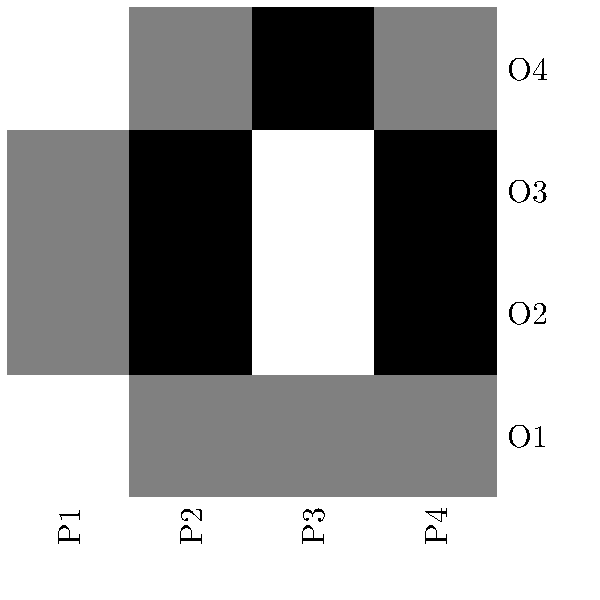
\includegraphics[width=0.3\textwidth]{fig-context-heatmap.pdf}
\caption{\label{fig:heatmap}The heatmap representing the formal context shown in Table~\ref{tab:fc}, obtained by doing \code{fc\$plot()}. A grey scale is used, where white indicates the value 0 for an object-attribute pair, while black indicates the value 1, with the greys representing the intermediate values. This type of graph aids visual inspection of the context, being able to check its sparsity, density or possible patterns.}
\end{figure}

\hypertarget{derivation-operators-1}{%
\subsection{Derivation operators}\label{derivation-operators-1}}

The methods that implement the derivation operators are named after
them: \code{intent()}, \code{extent()} and \code{closure()}. They can be
applied on objects of type \code{"Set"}, representing fuzzy sets of
objects or attributes:

\begin{example}
> S <- Set$new(fc$objects, O1 = 1, O2 = 1)
> S
{O1, O2}
> fc$intent(S)
{P2 [0.5], P4 [0.5]}
> T <- Set$new(fc$attributes, P1 = 1, P3 = 1)
> T
{P1, P3}
> fc$extent(T)
{}
> fc$closure(T)
{P1, P2, P3, P4}
\end{example}

In addition, we can perform \emph{clarification} on the formal context,
by using \code{fc\$clarify()}, giving:

\begin{example}
FormalContext with 3 objects and 3 attributes.
           P1   P3  [P2, P4]
       O1  0   0.5     0.5
       O4  0    1      0.5
 [O2, O3] 0.5   0       1
\end{example}

The duplicated rows and columns in the formal context have been
collapsed, and the corresponding attributes and objects' names are
grouped together between brackets, e.g., {[}P2, P4{]}.

\hypertarget{concept-lattice}{%
\subsection{Concept lattice}\label{concept-lattice}}

The command to compute the concept lattice for a \code{"FormalContext"}
\code{fc} is \code{fc\$find\_concepts()}. The lattice is stored in
\code{fc\$concepts}, which is of the \code{"ConceptLattice"} class.

\begin{example}
> fc$concepts
A set of 8 concepts:
1: ({O1, O2, O3, O4}, {P2 [0.5], P4 [0.5]})
2: ({O1, O4}, {P2 [0.5], P3 [0.5], P4 [0.5]})
3: ({O1 [0.5], O4}, {P2 [0.5], P3, P4 [0.5]})
4: ({O1 [0.5], O2, O3, O4 [0.5]}, {P2, P4})
5: ({O1 [0.5], O4 [0.5]}, {P2, P3, P4})
6: ({O2, O3}, {P1 [0.5], P2, P4})
7: ({O2 [0.5], O3 [0.5]}, {P1, P2, P4})
8: ({}, {P1, P2, P3, P4})
\end{example}

In order to know the \dfn{cardinality} of the set of concepts (that is,
the number of concepts), we can use \code{fc\$concepts\$size()}, which
gives 8 in this case. The complete list of concepts can be printed with
\code{fc\$concepts\$print()}, or simply \code{fc\$concepts}. Also, they
can be translated to \LaTeX{} using the \code{to\_latex()} method,
as mentioned before.

The typical subsetting operation in R with brackets is implemented to
select specific concepts from the lattice, giving their indexes or a
boolean vector indicating which concepts to keep. The same rules for
subsetting as in R base apply:

\begin{example}
> fc$concepts[c(1:3, 5, 8)]
A set of 5 concepts:
1: ({O1, O2, O3, O4}, {P2 [0.5], P4 [0.5]})
2: ({O1, O4}, {P2 [0.5], P3 [0.5], P4 [0.5]})
3: ({O1 [0.5], O4}, {P2 [0.5], P3, P4 [0.5]})
4: ({O1 [0.5], O4 [0.5]}, {P2, P3, P4})
5: ({}, {P1, P2, P3, P4})
\end{example}

In addition, the user can compute concepts' \dfn{support} (the
proportion of objects whose set of attributes contains the intent of a
given concept) by means of \code{fc\$concepts\$support()}.

\begin{example}
> fc$concepts$support()
[1] 1.00 0.50 0.25 0.50 0.00 0.50 0.00 0.00
\end{example}

\hypertarget{sublattices}{%
\subsubsection{Sublattices}\label{sublattices}}

When the concept lattice is too large, it can be useful to work with a
sublattice of the complete lattice on certain occasions. To this end, we
use the \code{sublattice()} function.

For instance, to build the sublattice generated by the concepts
\(\ensuremath{\left(\ensuremath{\left\{{^{0.5}}\!/\mathrm{O1},\, {^{0.5}}\!/\mathrm{O4}\right\}}, \ensuremath{\left\{\mathrm{P2},\, \mathrm{P3},\, \mathrm{P4}\right\}}\right)}\)
and
\(\ensuremath{\left(\ensuremath{\left\{\mathrm{O2},\, \mathrm{O3}\right\}}, \ensuremath{\left\{{^{0.5}}\!/\mathrm{P1},\, \mathrm{P2},\, \mathrm{P4}\right\}}\right)}\),
which had indexes 5 and 6 in the list of concepts, we can do:

\begin{example}
> fc$concepts$sublattice(5:6)
A set of 4 concepts:
1: ({O1 [0.5], O2, O3, O4 [0.5]}, {P2, P4})
2: ({O1 [0.5], O4 [0.5]}, {P2, P3, P4})
3: ({O2, O3}, {P1 [0.5], P2, P4})
4: ({}, {P1, P2, P3, P4})
\end{example}

Some interesting sublattices appear when we consider only concepts
fulfilling a given condition (e.g., a minimum support), using a command
such as \code{fc\$concepts\$sublattice(fc\$concepts\$support() >\ 0.5)}.

\hypertarget{subconcepts-superconcepts-infimum-and-supremum}{%
\subsubsection{Subconcepts, superconcepts, infimum and
supremum}\label{subconcepts-superconcepts-infimum-and-supremum}}

For a given concept \((A, B)\), we can find all its subconcepts
(\((C_i, D_i)\) such that \((C_i, D_i)\le (A, B)\)) by using the
\code{subconcepts()} functions. Analogously, the \code{superconcepts()}
function can be used to compute the set of \((C_i, D_i)\) such that
\((A, B) \le (C_i, D_i)\).

For instance, if we take a sample concept \(L=\)
\ensuremath{\left(\ensuremath{\left\{{^{0.5}}\!/\mathrm{O1},\, \mathrm{O2},\, \mathrm{O3},\, {^{0.5}}\!/\mathrm{O4}\right\}}, \ensuremath{\left\{\mathrm{P2},\, \mathrm{P4}\right\}}\right)}
, we can compute its subconcepts and superconcepts using:

\begin{example}
> fc$concepts$subconcepts(L)
A set of 5 concepts:
1: ({O1 [0.5], O2, O3, O4 [0.5]}, {P2, P4})
2: ({O1 [0.5], O4 [0.5]}, {P2, P3, P4})
3: ({O2, O3}, {P1 [0.5], P2, P4})
4: ({O2 [0.5], O3 [0.5]}, {P1, P2, P4})
5: ({}, {P1, P2, P3, P4})
> fc$concepts$superconcepts(L)
A set of 2 concepts:
1: ({O1, O2, O3, O4}, {P2 [0.5], P4 [0.5]})
2: ({O1 [0.5], O2, O3, O4 [0.5]}, {P2, P4})
\end{example}

Also, we can define the infimum and the supremum of a set of concepts as
the greatest common subconcept and the lowest common superconcept of all
the given concepts, respectively. For a list of concepts, we can compute
its infimum and supremum using the \code{supremum()} and
\code{infimum()} methods of the \code{"ConceptLattice"} object. Additionally, irreducible elements in the lattice, with respect to join
(supremum) and meet (infimum), can be computed for a given concept
lattice with the methods \code{join\_irreducibles()} and
\code{meet\_irreducibles()}.

\begin{example}
> fc$concepts$meet_irreducibles()
A set of 5 concepts:
1: ({O1, O4}, {P2 [0.5], P3 [0.5], P4 [0.5]})
2: ({O1 [0.5], O4}, {P2 [0.5], P3, P4 [0.5]})
3: ({O1 [0.5], O2, O3, O4 [0.5]}, {P2, P4})
4: ({O2, O3}, {P1 [0.5], P2, P4})
5: ({O2 [0.5], O3 [0.5]}, {P1, P2, P4})
> fc$concepts$join_irreducibles()
A set of 5 concepts:
1: ({O1, O4}, {P2 [0.5], P3 [0.5], P4 [0.5]})
2: ({O1 [0.5], O4}, {P2 [0.5], P3, P4 [0.5]})
3: ({O1 [0.5], O4 [0.5]}, {P2, P3, P4})
4: ({O2, O3}, {P1 [0.5], P2, P4})
5: ({O2 [0.5], O3 [0.5]}, {P1, P2, P4})
\end{example}

These irreducible elements are essential since they constitute the basic
elements with which the entire concept lattice can be reconstructed.

\hypertarget{the-standard-context}{%
\subsubsection{The standard context}\label{the-standard-context}}

The standard context has a concept lattice that is isomorphic to the one
of the original context, so it encapsulates the same knowledge. With
\pkg{fcaR} one can directly compute the standard context by using the
\code{standardize()} function, for example, using
\code{fc\_std <-\ fc\$standardize()} to save the new context to another
variable.

This is a method that applies to a \code{"FormalContext"} object, but is
closely related to its associated \code{"ConceptLattice"}, since the
objects and attributes of the newly created standard context are the
meet- and join- irreducible elements of the concept lattice.

The standard context for the example in Table~\ref{tab:fc} and its
corresponding lattice are shown in Table~\ref{tab:std}.

\begin{table}

\begin{tabular}{cc}
\begin{minipage}{0.40\linewidth}
    \centering
    \small

\begin{tabular}{lccccc} \toprule  & M1 & M2 & M3 & M4 & M5\\ \midrule J1 & $\times$ &   &   &   &  \\  J2 & $\times$ & $\times$ &   &   &  \\  J3 & $\times$ & $\times$ & $\times$ &   &  \\  J4 &   &   & $\times$ & $\times$ &  \\  J5 &   &   & $\times$ & $\times$ & $\times$\\ \bottomrule \end{tabular}

  \end{minipage}
  &

\begin{minipage}{0.50\linewidth}

\centering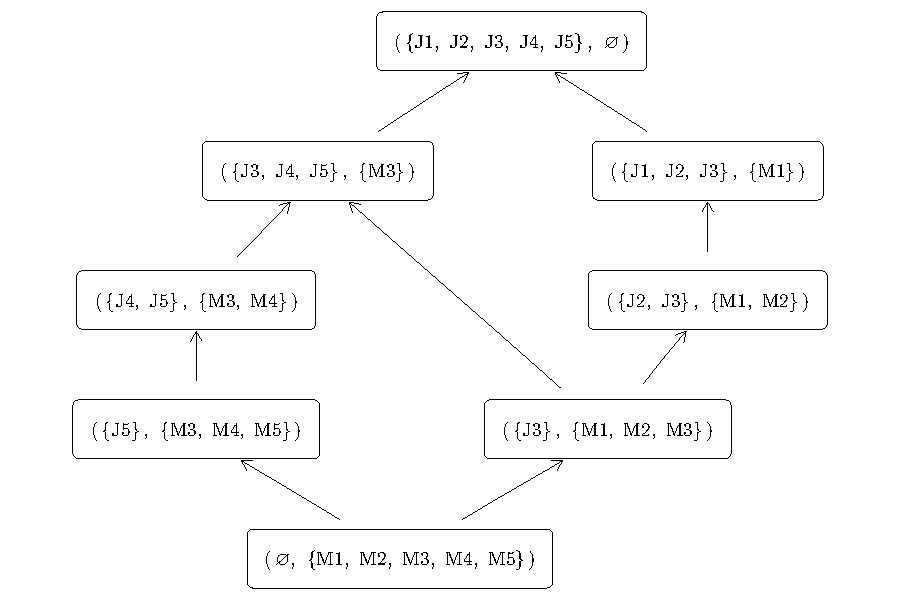
\includegraphics[width=\linewidth]{fig-std-lattice.pdf}


\end{minipage} \\
\end{tabular}
\caption{Left: Standard context associated to the context in Table~\ref{tab:fc}; M1 to M5 refer to the meet-irreducible elements of the formal context, and J1 to J5, to the join-irreducible ones. Right: concept lattice of the standard context, isomorphic to the one in Figure~\ref{fig:lattice}.}\label{tab:std}
\end{table}

\hypertarget{implications-and-logic-1}{%
\subsection{Implications and logic}\label{implications-and-logic-1}}

As mentioned earlier, a core problem in FCA is the computation of
implications that hold in a formal context. The iterative fuzzy version
of \textsc{NextClosure} has been implemented in C and made accessible
from \pkg{fcaR} thanks to an interface using \pkg{Rcpp}. As we have
said, our package can manage classical implications from binary
datasets. In order to build the Duquenne-Guigues basis of implications,
by using the \textsc{NextClosure} algorithm, the command
\code{fc\$find\_implications()} is executed, and the result is stored in
\code{fc\$implications}.

The set of implications is stored as an object of class
\code{"ImplicationSet"}, which can be inspected with the \code{print()}
method or simply with \code{fc\$implications}. In order to get a subset
of the implications by providing its indexes, the standard R subsetting
with \samp{[} will create another \code{"ImplicationSet"} with exactly
the rules required. For instance, \code{fc\$implications[1:3]} gives:

\begin{example}
Implication set with 3 implications.
Rule 1: {} -> {P2 [0.5], P4 [0.5]}
Rule 2: {P2 [0.5], P4} -> {P2}
Rule 3: {P2, P4 [0.5]} -> {P4}
\end{example}

These implications can be converted to \LaTeX~using the
\code{to\_latex()} method, giving:

\begingroup\footnotesize

\begin{longtable*}{rrcl}
1: &\ensuremath{\varnothing}&\ensuremath{\Rightarrow}&\ensuremath{\left\{{^{0.5}}\!/\mathrm{P2},\, {^{0.5}}\!/\mathrm{P4}\right\}}\\
2: &\ensuremath{\left\{{^{0.5}}\!/\mathrm{P2},\, \mathrm{P4}\right\}}&\ensuremath{\Rightarrow}&\ensuremath{\left\{\mathrm{P2}\right\}}\\
3: &\ensuremath{\left\{\mathrm{P2},\, {^{0.5}}\!/\mathrm{P4}\right\}}&\ensuremath{\Rightarrow}&\ensuremath{\left\{\mathrm{P4}\right\}}\\
\end{longtable*}\endgroup

On the other hand, one can \code{filter()} the implications to retrieve
just those with specific attributes in the LHS and RHS. As before, the
method returns a new \code{"ImplicationSet"} object. For example, to get the implications with attributes P1 and P2 in the
LHS and attribute P4 in the RHS, the user can execute
\code{fc\$implications\$filter(lhs =\ c('P1',\ 'P2'),\ rhs =\ 'P4')}.

Some quantities can be computed from a set of implications:

\begin{itemize}
\tightlist
\item
  \dfn{Cardinality}, that is, the number of implications, with
  \code{fc\$implications\$cardinality()}.
\item
  \dfn{Size}, which is the cardinality of the LHS and RHS of
  \textit{each} implication, interpreted as fuzzy sets (thus non-integer
  sizes can appear): \code{fc\$implications\$size()}.
\item
  \dfn{Support}, the proportion of objects in the formal context whose
  set of attributes is a \emph{superset} of the LHS of each implication:
  \code{fc\$implications\$support()}.
\end{itemize}

\clearpage

\hypertarget{application-of-the-simplification-logic}{%
\subsubsection{Application of the simplification
logic}\label{application-of-the-simplification-logic}}

In \pkg{fcaR}, the simplification logic has been implemented and made
accessible from an \code{"ImplicationSet"} object through method
\code{apply\_rules}.

The list of equivalence rules applicable to an \code{"ImplicationSet"}
is stored in a \code{registry} object from the \CRANpkg{registry}
package by \citet{registry}.

This registry is called \code{equivalencesRegistry}, and one can inspect
its contents by using:

\begin{example}
> equivalencesRegistry$get_entry_names()
[1] "Composition"          "Generalization"       "Reduction"
[4] "Simplification"       "Right Simplification" "Reorder"
\end{example}

These names correspond to the methods added to the registry by default
and are used to index those methods. Every method is accompanied by a
description, so that we can see its definition:

\begin{example}
> equivalencesRegistry$get_entry('Composition')
     method Composition
        fun <<function>>
description A -> B and A -> C equivalent to A -> BC
\end{example}

We can even use abbreviated names to refer to the method. For instance,
we can use \samp{comp} instead of \samp{Composition} in the above
command to obtain the information about the composition rule.

The registry's use enables the user to extend the functionality provided
by the \pkg{fcaR} package. One can define and implement new equivalences
rules and add them to the registry, and make them available to the
\code{apply\_rules()} method.

In order to add a new equivalence rule, we use the following:

\begin{example}
> equivalencesRegistry$set_entry(method = 'Method name',
+                                fun = method_function,
+                                description = 'Method description')
\end{example}
where \code{method\_function()} is the R function that computes the
equivalences, and has the signature
\code{function(LHS, RHS, attributes)}, where \code{LHS} and \code{RHS}
are the sparse matrices defining the left-hand and right-hand sides of
the implications, \code{attributes} is the character vector of attribute
names, and returns the modified \code{LHS} and \code{RHS}. This
mechanism has been used in the package to implement additional
equivalence rules.

The user can decide which rules to remove redundancies will be applied
and in which order:

\begin{example}
> fc$implications$apply_rules(rules = c('reduction',
+                                       'comp',
+                                       'gener',
+                                       'simpl'))
\end{example}

These methods can be applied to binary and fuzzy implications.

\hypertarget{computation-of-closure-and-recommendations}{%
\subsubsection{Computation of closure and
recommendations}\label{computation-of-closure-and-recommendations}}

One of the primary uses of a set of implications extracted from a formal
context is computing the closure of a set of attributes, that is, the
fuzzy set obtained by applying the given implications on the set of
attributes.

The \code{closure()} method returns both the closure and the reduced
\code{"ImplicationSet"} if \code{reduce = TRUE} and only the closure if
\code{reduce = FALSE} (default). For instance, we can create a fuzzy set
where the attribute \code{P2} is present with:

\begin{example}
> A <- Set$new(attributes = fc$attributes, P2 = 1)
\end{example}

Then, we can compute its closure and the reduced set of implications
doing:

\begin{example}
> fc$implications$closure(A, reduce = TRUE)
$closure
{P2, P4}

$implications
Implication set with 2 implications.
Rule 1: {P3 [0.5]} -> {P3}
Rule 2: {P1 [0.5], P3} -> {P1}
\end{example}

\hypertarget{examples}{%
\section{Usage example. Fuzzy diagnostic system}\label{examples}}

In this section, a complete example of the use of \pkg{fcaR} on
real-world problems is presented: Designing a diagnostic system from a
formal context with (fuzzy) medical data.

The dataset for this section is provided and documented in the package.

In this example, the aim is to build an automated system using the
\pkg{fcaR} package to perform medical diagnosis. We have focused on
neurological pathologies since, in recent years, an increasing number of
initiatives have appeared to share, curate, and study specific,
prevalent brain pathologies. Among these pathologies, schizophrenia is
of the highest interest, and public, curated repositories have been
released.

The data source is SchizConnect \citep{wang2016schizconnect}, an online
data repository integrating and mediating data from other
schizophrenia-related databases, such as COBRE
\citep{aine2017multimodal}, which collect neuroimaging, psychological,
neurological and clinical information. SchizConnect allows retrieving
data about the patients that fulfil some conditions introduced as a
query to the database. A subset of the COBRE dataset has been retrieved
by querying SchizConnect for 105 patients with neurological and clinical
symptoms. We also collected their corresponding diagnosis.

Among the clinical attributes in the dataset, one can find:

\begin{itemize}
\tightlist
\item
  \emph{Calgary Depression Scale for Schizophrenia}
  \citep{addington1990depression}, nine items (attributes) assessing the
  level of depression in schizophrenia, differentiating between positive
  and negative aspects of the disease.
\item
  The \emph{Simpson-Angus Scale} \citep{simpson1970rating}, six items to
  evaluate Parkinsonism-like alterations related to schizophrenia in an
  individual.
\item
  The \emph{Structured Clinical Interview for DSM-III-R Personality
  Disorders} \citep{first1997user}, with nine variables related to the
  presence of signs affecting personality.
\item
  The diagnosis for each individual: it can be \emph{schizophrenia
  strict} (abbreviated \samp{dx\_ss}) or \emph{other diagnosis}
  (abbreviated \samp{dx\_other}, which includes schizoaffective and
  bipolar disorders). These diagnoses are mutually exclusive; thus, only
  one of them is assigned to each patient.
\end{itemize}

In summary, the dataset consists of the previous 30 attributes related
to signs or symptoms and two attributes related to diagnosis. So the
dataset has 105 objects (patients), and 32 attributes to explore. The
symptom attributes are multi-valued.

For a given attribute (symptom), the available grades are \emph{absent},
\emph{minimal}, \emph{mild}, \emph{moderate}, \emph{moderate severe},
\emph{severe} and \emph{extreme}. Thus, taking into account these scale
levels, the attributes are coded as fuzzy and graded attributes with
values 0, \(\sfrac{1}{6}\), \(\sfrac{1}{3}\), \(\sfrac{1}{2}\),
\(\sfrac{2}{3}\), \(\sfrac{5}{6}\) and 1, respectively. Since the symptom attributes are ordinal, for the sake of simplicity, they have been encoded as grades in the interval $[0, 1]$, just by mapping the lowest (\emph{absent}) value to 0 and the greatest (\emph{extreme}) to 1 and placing the remaining values equidistantly in the interval. In~\citet{ganter2016conceptual},  other strategies of scaling for ordinal, nominal, or interval attributes are presented.

%%% Last sentence added as a response to reviewer 1.

In \pkg{fcaR}, this dataset is exposed to the user with the name
\code{cobre32}, and we can use it to create a fuzzy formal context (see
Figure~\ref{fig:schizo}):

\begin{example}
> fc <- FormalContext$new(cobre32)
\end{example}

\begin{figure}[t]
\centering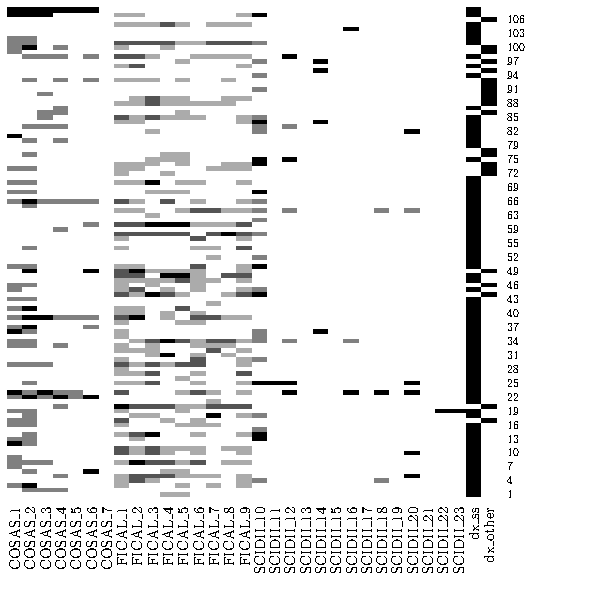
\includegraphics[width=0.7\linewidth]{formal_context.pdf}
\caption{\label{fig:schizo}Formal context of the \code{cobre32} dataset. The default plot type allows us to identify patterns occurring in the attributes, such as the sparsity of the \code{SCIDII} variables. Additionally, we can see that the variables indicating diagnosis, \code{dx\_ss} and \code{dx\_other} in the last two columns, are binary and mutually exclusive.}
\end{figure}

Now, let us build a diagnosis system that employs the tacit knowledge
present in the formal context. The objective is to define a function
that takes a \code{"Set"} as input (with the clinical attributes of an
individual) and returns the degree of the diagnosis attributes using the
implications extracted from the formal context as an inference engine.

Next, we use the \textsc{NextClosure} algorithm to extract implications
and compute the set of concepts, using \code{fc\$find\_implications()}.

The concept lattice is quite big (14706 concepts); therefore, it cannot
be plotted here for space and readability reasons. For this reason, we
only plot a sublattice of small size in
Figure~\ref{fig:sublatticecobre32}.

\begin{figure}[t]
\centering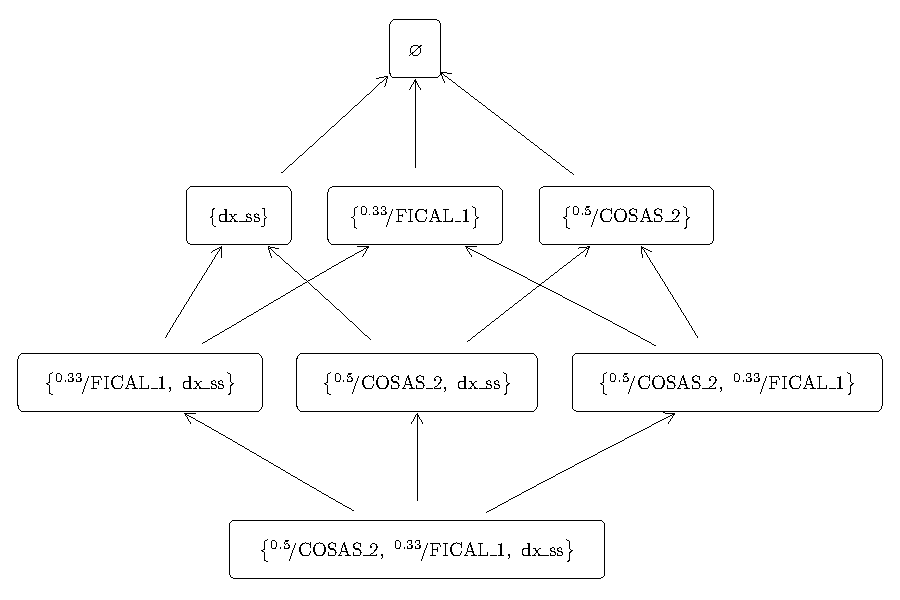
\includegraphics[width=0.6\linewidth]{fig-sublatticecobre32.pdf}
\caption{\label{fig:sublatticecobre32}Hasse diagram for a sublattice of the \code{cobre32} formal context. Since the complete concept lattice is huge, with the Hasse diagram of a sublattice we can understand the relationship in a subset of the attributes. In this case, we can see how variables \code{COSAS\_2} and \code{FICAL\_1} are related to the variable \code{dx\_ss} which indicates the schizophrenia diagnosis.}
\end{figure}

There is an aggregate of 985 implications extracted. Let us compute the
average cardinality of the LHS and the RHS of the extracted rules:

\begin{example}
> colMeans(fc$implications$size())
     LHS      RHS
2.417597 1.954146
\end{example}

Note that our paradigm can deal with non-unit implications, that is,
where there is more than one attribute in the RHS of the implication.
This feature is an extension of what is usual in other paradigms, for
example, in transactional databases.

We can use the \emph{simplification logic} to remove redundancies and
reduce the LHS and RHS size of the implications. The reason to do this
is to decrease the computational cost of computing closures:

\begin{example}
> fc$implications$apply_rules(rules = c('simplification', 'rsimplification'))
> colMeans(fc$implications$size())
     LHS      RHS
1.998308 1.557191
\end{example}

We can see that the average cardinality of the LHS has been reduced from
2.418 to 1.998 and that the one of the RHS, from 1.954 to 1.557.

With the simplified implication set, we can build a recommender system
by simply wrapping the \code{recommend()} method inside a function:

\begin{example}
> diagnose <- function(S) {
+
+   fc$implications$recommend(S = S,
+                             attribute_filter =
+                               c('dx_ss', 'dx_other'))
+
+ }
\end{example}

This function can be applied to \code{"Set"}s that have the same
attributes as those of the formal context. The \code{attribute\_filter}
argument specifies which attributes are of interest, in our case, the
diagnosis attributes.

Let us generate some sets of attributes and get the recommendation
(diagnosis) for each one:

\begin{example}
> S1 <- Set$new(attributes = fc$attributes,
+               COSAS_1 = 1/2, COSAS_2 = 1, COSAS_3 = 1/2,
+               COSAS_4 = 1/6, COSAS_5 = 1/2, COSAS_6 = 1)
> diagnose(S1)
   dx_ss dx_other
       1        0
> S2 <- Set$new(attributes = fc$attributes,
+               COSAS_2 = 1, COSAS_6 = 1, FICAL_1 = 1/3, FICAL_3 = 1/3)
> diagnose(S2)
   dx_ss dx_other
       0        0
> S3 <- Set$new(attributes = fc$attributes,
+               COSAS_4 = 2/3, FICAL_3 = 1/2, FICAL_5 = 1/2, FICAL_8 = 1/2)
> diagnose(S3)
   dx_ss dx_other
       0        1
\end{example}

These results mean that, for \code{S1}, the recommended diagnosis is
schizophrenia strict, for \code{S2} there is not enough information, and
the recommended diagnosis for \code{S3} is \emph{other}, different from
schizophrenia strict. For \code{S2}, maybe adding more attributes to it
can help in obtaining a diagnosis.

One can inspect the reduced set of implications obtained after computing
the closure for \code{S2}, simplify them and filter them to get the
implications that can be applied if more attribute values are known for
\code{S2}:

\begin{example}
> cl <- fc$implications$closure(S2, reduce = TRUE)
> cl$implications$apply_rules(c('simp', 'rsimp', 'reorder'))
> cl$implications$filter(rhs = c('dx_ss', 'dx_other'),
+                        not_lhs = c('dx_ss', 'dx_other'), drop = TRUE)
Implication set with 12 implications.
Rule 1: {FICAL_5 [0.33]} -> {dx_other}
Rule 2: {FICAL_6 [0.33], FICAL_8 [0.33]} -> {dx_ss}
Rule 3: {SCIDII_18 [0.33]} -> {dx_ss}
Rule 4: {COSAS_1 [0.5], FICAL_8 [0.33]} -> {dx_ss}
Rule 5: {SCIDII_20 [0.33]} -> {dx_ss}
Rule 6: {SCIDII_16 [0.33]} -> {dx_ss}
Rule 7: {SCIDII_12 [0.33]} -> {dx_ss}
Rule 8: {FICAL_7 [0.33]} -> {dx_ss}
Rule 9: {FICAL_6 [0.33], SCIDII_10 [0.5]} -> {dx_ss}
Rule 10: {COSAS_3 [0.5]} -> {dx_ss}
Rule 11: {COSAS_1 [0.5]} -> {dx_ss}
Rule 12: {SCIDII_10 [0.5]} -> {dx_ss}
\end{example}

We can check that, for \code{S2}, if the presence of any symptom (of the
LHS of the implications) is verified, then the implications above could
directly tell us the diagnosis.

An extended version of the diagnosis system in this example has been
presented in \citet{CORDERO2020113449}, where the \pkg{fcaR} package
has been used to build a conversational recommender system based on
fuzzy rules. In that work, the recommender system designed with the help
of \pkg{fcaR} has obtained better results than those of the classical
methods used in the area of recommendations.

\hypertarget{conclusions}{%
\section{Conclusions and future work}\label{conclusions}}

This work aims to present the first R package implementing the core
methods in Formal Concept Analysis. This development aims to provide a
helpful tool for the FCA community and other fields where knowledge
discovery and retrieval play an essential role. Notably, the
hybridization of FCA with other Machine Learning techniques and its
application to data mining processes is well-known, making FCA an
appealing tool for knowledge discovery.

This package provides \pkg{R6} classes and methods to manage datasets
presented as formal contexts, use the derivation operators, work with
the concepts (closed itemsets) or find and manage the basis of
implications. Additionally, the \pkg{fcaR} package implements a logic to
infer knowledge from sets of implications, allowing to compute closures
and therefore, it can be used as the engine to build recommender systems
and automated reasoning tools.

Another feature included in the package is providing graphical
visualisations of the concept lattice that condenses the extracted
knowledge.

The tool has been developed from two principles: \emph{integration} with
other packages and \emph{extensibility}. First, the \pkg{arules} package
is a \emph{de facto} standard when working with transactional databases,
closed itemsets and association rules in R. Since FCA's perspective can
be seen as complementary to this, \pkg{fcaR} is able to import and
export both the datasets and the implications from/to the analogous
classes defined in \pkg{arules}. This way, the user of \pkg{arules} can
benefit from the FCA tools in \pkg{fcaR}, including the simplification
logic.

The extensibility of the \pkg{fcaR} is guaranteed by its design
philosophy. First, the object-oriented programming paradigm allows
extending the classes and methods to other datatypes, other kinds of
formal contexts, or, for example, association rules. Second, using a
registry for equivalence rules makes it easy to include new logic tools
in the package's architecture without affecting existing code. Thus,
users can extend the package's functionality by incorporating their
methods and then testing and comparing them in a single framework.

Thus, \pkg{fcaR} implements a wide range of features. With the help of
the included documentation and the comprehensive vignettes, any user can
start analysing datasets with FCA tools quickly.

Regarding the low-level implementation, we have used sparse matrices as
the primary internal data structure of the package since they represent
a space- and cost-efficient storage. Also, when needed, the \pkg{fcaR}
uses parallel computing and C routines to increase efficiency and tackle
algorithmic bottlenecks.

As an example of use, we have used the implications extracted from a
dataset to develop a recommender system to help diagnose schizoaffective
disorders quickly.

The package is currently in stable development status. However, we
devise future extensions in terms of new or improved algorithms or as
new applications arise (in areas such as recommender systems,
unsupervised learning or text mining).

We emphasize that \pkg{fcaR} is having a great acceptance. At the time
of writing, it has now reached more than 20,000 downloads from CRAN.

\section*{Acknowledgments}

This work has been partially supported by the projects TIN2017-89023-P
(Spanish Ministry of Economy and Competitiveness, including FEDER
funds), PGC2018-095869-B-I00 (Spanish Ministry of Science and
Innovation), and the Junta de Andalucía project UMA2018-FEDERJA-001,
co-funded by the European Regional Development Fund.

\bibliography{fcaR.bib}

\address{%
Pablo Cordero\\
Universidad de Málaga\\%
Departamento de Matemática Aplicada\\ ETSI Telecomunicaciones, Campus de
Teatinos\\
%
\url{http://webpersonal.uma.es/de/pcordero/My_personal_web/Wellcome.html}%
\\\textit{ORCiD: \href{https://orcid.org/0000-0002-5506-6467}{0000-0002-5506-6467}}%
\\\href{mailto:pcordero@uma.es}{\nolinkurl{pcordero@uma.es}}
}

\address{%
Manuel Enciso\\
Universidad de Málaga\\%
Departamento de Lenguajes y Ciencias de la Computación\\ ETSI
Informática, Campus de Teatinos\\
%
\url{http://lcc.uma.es/~enciso/index_EN.html}%
\\\textit{ORCiD: \href{https://orcid.org/0000-0002-0531-4055}{0000-0002-0531-4055}}%
\\\href{mailto:enciso@uma.es}{\nolinkurl{enciso@uma.es}}
}

\address{%
Domingo López-Rodríguez\\
Universidad de Málaga\\%
Departamento de Matemática Aplicada\\ ETSI Telecomunicaciones, Campus de
Teatinos\\
%
\url{https://dominlopez.netlify.app}%
\\\textit{ORCiD: \href{https://orcid.org/0000-0002-0172-1585}{0000-0002-0172-1585}}%
\\\href{mailto:dominlopez@uma.es}{\nolinkurl{dominlopez@uma.es}}
}

\address{%
Ángel Mora\\
Universidad de Málaga\\%
Departamento de Matemática Aplicada\\ ETSI Informática, Campus de
Teatinos\\
%
\url{https://amorabonilla.github.io/}%
\\\textit{ORCiD: \href{https://orcid.org/0000-0003-4548-8030}{0000-0003-4548-8030}}%
\\\href{mailto:amora@uma.es}{\nolinkurl{amora@uma.es}}
}
